\chapter{Prototipo final}\label{protof}

Con el prototipo anterior, se logra una base con la cual ya implementar el servidor web al cual conectarse. No sin antes analizar posibles mejoras a lo ya hecho, en base a distintas pruebas de rendimiento y cambios menores principalmente a nivel de comunicación Bluetooth.

En las siguientes seccioness se detallan los cambios realizados para el prototipo final, en donde se destacan mejoras necesarias de la versión 2 y la selección e implementación del servidor web.

\section{Paquetes de control Bluetooth}

A partir de la segunda versión del prototipado, se pudo observar cierta tasa de error no menor en la recepción de comandos por parte del microcontrolador. Esto debido a la cantidad de operaciones hechas por segundo y ciertas respuestas de parte del módulo Bluetooth que no son homogéneas, complejizando así su detección.

Por esta razón y para no esperar una medición errónea (realizar una petición de cierto sensor y que el microcontrolador ejecute la medición pero de otro sensor) se implementa un mensaje de confirmación por parte del microcontrolador: Luego de la petición hacia el módulo Bluetooth, esta petición se procesa y confirma de vuelta hacia la aplicación, la cual analiza la respuesta y toma la decisión de reenviar la petición (en caso de que se haya considerado errónea) o ejecutarla (en caso de considerarla correcta).

Lo anterior, por medio de un mensaje con la cadena de texto ``AAAA" seguido de 2 caracteres asociados a los sensores: ``01",``11",``10".

\section{Implementación de Realm}

Ya hechas las mejoras pertinentes a la programación del microcontrolador, se comienzan a implementar nuevas funciones a la aplicación, como lo es su base de datos local.

Como ya se mencionó en el capítulo anterior, la base de datos seleccionada es Realm. Respecto al modelo presentado se simplifican las tablas \ref{tabla_datos_T} y \ref{tabla_datos_ECG} por la posibilidad de generar un arreglo contenido en una medición de T y ECG respectivamente. 

El manejo de las tablas en Realm se hace sencilla por su símil con los objetos en Java, al poder extender clases desde RealmObject y tratarlos como cualquier objeto pero utilizable en conjunto con Realm. Además de lo anterior, existe un tipo específico para listas de estos objetos (RealmList) con la cual se puede omitir las tablas ya mencionadas y agrupar esos datos (en forma de una lista) dentro de un RealmObject asociado a cada medición.

\begin{figure}[H]
	\centering
	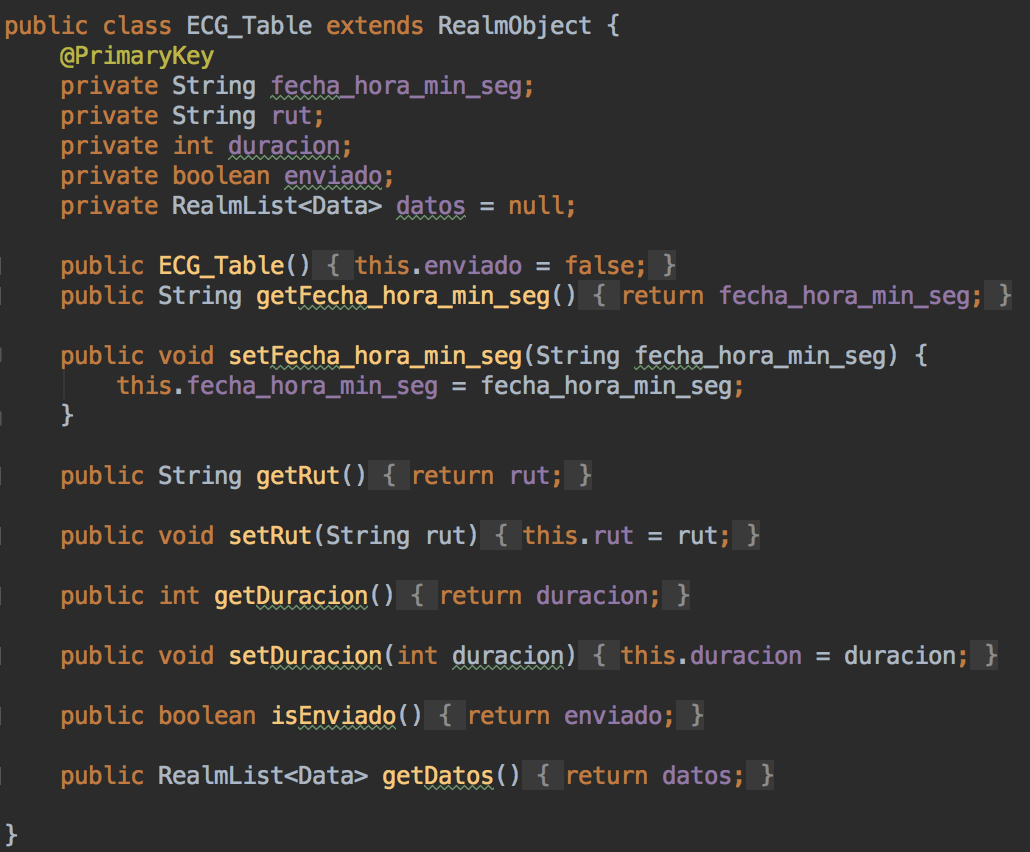
\includegraphics[scale=0.6]{figuras/protof/realmobject.png}
	\caption{Clases de Realm utilizados para los datos de ECG}
	\label{realm_ecg}
\end{figure}

Pensando en la comunicación de los datos y dado que se está trabajando con objetos en Java para las distintas tablas y datos, es importante implementar algún método para serializar los datos, específicamente a JSon por su amplia utilización actual. Esto pensando en la comunicación final con el servidor tanto para los casos de comunicación en vivo como para los casos de sincronización entre bases de datos. Para esto último se utiliza la librería GSon de Google, la cual simplifica la implementación de JSon a partir de objetos.

Además de lo anterior ya expuesto, solo se ha seguido la guía oficial de Realm para su implementación en Android, por lo que se omite esta información por ser de común lectura \cite{realm_android}.


\section{Servicio web}

Si bien en capítulos anteriores se implementó un servidor web basado en Python (Tornado), se descarta su uso por el acelerado proceso de desarrollo que se requiere, la pobre documentación que posee y las pocas ayudas frente al desarrollo de interfaces usuarias amigables o sencillas.

Por lo anterior y pensando en un cambio completo del servicio web, se buscan entre distintas alternativas que sean compatibles con los requerimientos del proyecto:

\textbf{Motor Web}: NodeJS (mongoose, socket.io, angularJS), MeteorJS, ExpressJS.

\textbf{Base de datos}: InfluxDB, FireBase, PostgreSQL.

\textbf{Visualización de datos}: Grafana, D3, High Charts, ChartsJS.

\textbf{Comunicación}: WebSocket.

Como se puede observar, la única seguridad de la cual el proyecto no se puede alejar es del uso de WebSocket
dadas sus prestaciones (alta velocidad y baja latencia).

\newpage


Analizando las distintas opciones ya mencionadas se determina configurar un servidor con las siguientes características:
 
 \textbf{Dominio}: Se adquiere por \$10.000 pesos en NIC (nombres de dominio CL) el dominio ``proyectogaleno.cl". Del cual se puede ver el certificado en los anexos.
 
\textbf{DNS}: De forma gratuita, se consigue con Namecheap (registrador acreditado por la ICANN (Internet Corporation for Assigned Names and Numbers) que brinda servicios de registro de nombres de dominio y ofrece nombres de dominio de venta que están registrados a terceros) bajo el domninio ``proyectogaleno.cl".

\textbf{Email}: Para no montar directamente un servidor de correos electrónicos, se configura una redirección por el mismo servicio de Namecheap hacia el dominio ya mencionado.

\textbf{Servidor Web}: MeteorJS, por su enfoque a las conexiones en tiempo real (con el uso de WebSocket), por ser FullStack basado en JavaScript permitiendo un ágil desarrollo y por poseer el repositorio AtmosphereJS, que cuenta con multitud de paquetes de toda índole y de rápida implementación.

\textbf{Websocket}: DDP, protocolo que define cierto estándar de comunicación entre el servidor y los clientes, con el uso de mensajes JSON sobre websocket. Haciendo realmente rápida la implementación de la comunicación sobre WebSocket.

\textbf{Librería gráfica JS}: D3, librería de JavaScript para producir, a partir de datos, infogramas dinámicos e interactivos en navegadores web, haciendo uso de tecnologías bien sustentadas como SVG, HTML5, y CSS. Su elección radica en el gran control final que otorga y su fácil implementación en conjunto con Meteor con su paquete oficial d3js:d3.

\textbf{Base de datos}: MongoDB, si bien se analizaron otras opciones, se sigue prefiriendo su uso por sus características base y por su buen acoplo con MeteorJS.

\textbf{Proxy reverso}: NGinx, en este apartado no se realizaron modificaciones pues no existe competencia real dadas las prestaciones que ofrece y los requerimientos del proyecto (pasando por los fondos disponibles). \newline

\textbf{Seguridad}: HTTPS y WSS (CertBot/LetsEncrypt), en este apartado se escoge utilizar certificados provistos gratuitamente por LetsEncrypt para hacer uso de los protocolos ya mencionados. HTTPS ofrece una base segura de intercambio de información entre el servidor y los clientes, sobre la cual además se utiliza WSS que es la versión encriptada de WS (protocolo de websocket). Dotando en conjunto de una segura comnunicación sin perder rendimiento, pues ambas técnicas se basan en una sobrecarga principalmente al iniciar la comunicación y no en cada mensaje intercambiado.

\begin{figure}[H]
	\centering
	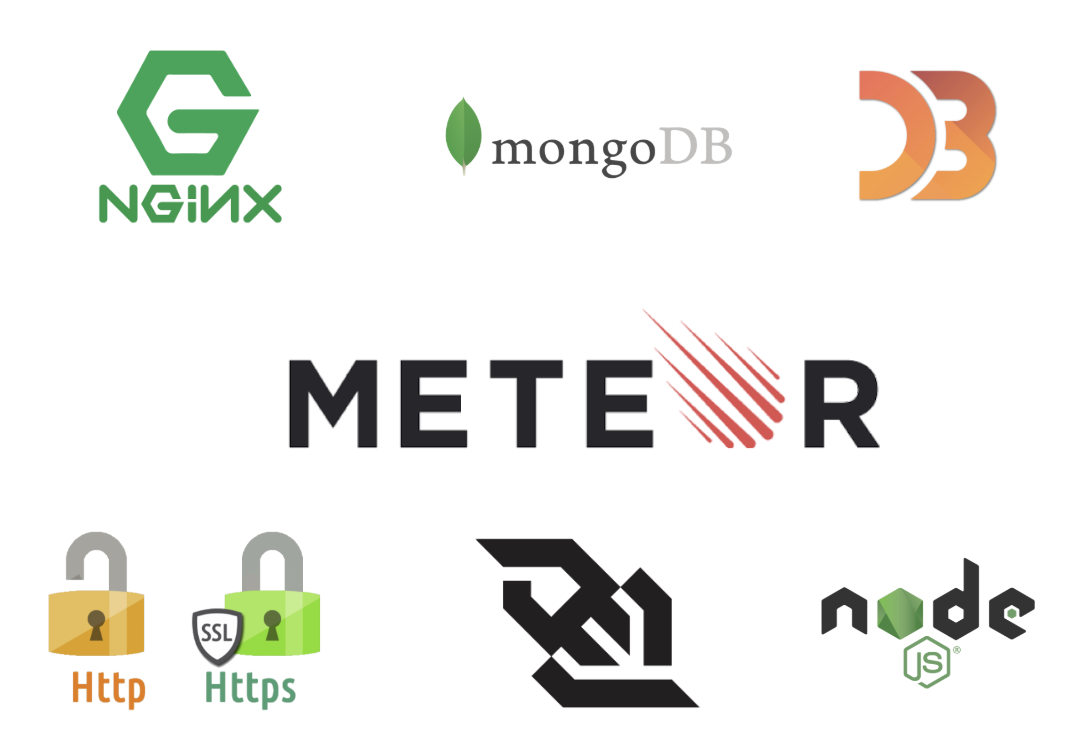
\includegraphics[scale=0.6]{figuras/protof/tecnologias.png}
	\caption{Tecnologías empleadas en el lado del servidor}
	\label{tecnologias}
\end{figure}


En la figura \ref{tecnologias} se pueden observar en conjunto y a grandes rasgos, las distinas tecnologías empleadas para dar soporte web al proyecto.

\newpage


\section{Selección de usuario, tipo de cuentas y muestras}

Dadas las caracetrísticas del proyecto, se articulan dos tipos de cuentas principales en una primera instancia: Normal, con la cual poder acceder solo a la visualización de datos y Total, con la cual se pueden realizar mediciones desde la misma web. 

\begin{figure}[H]
	\centering
	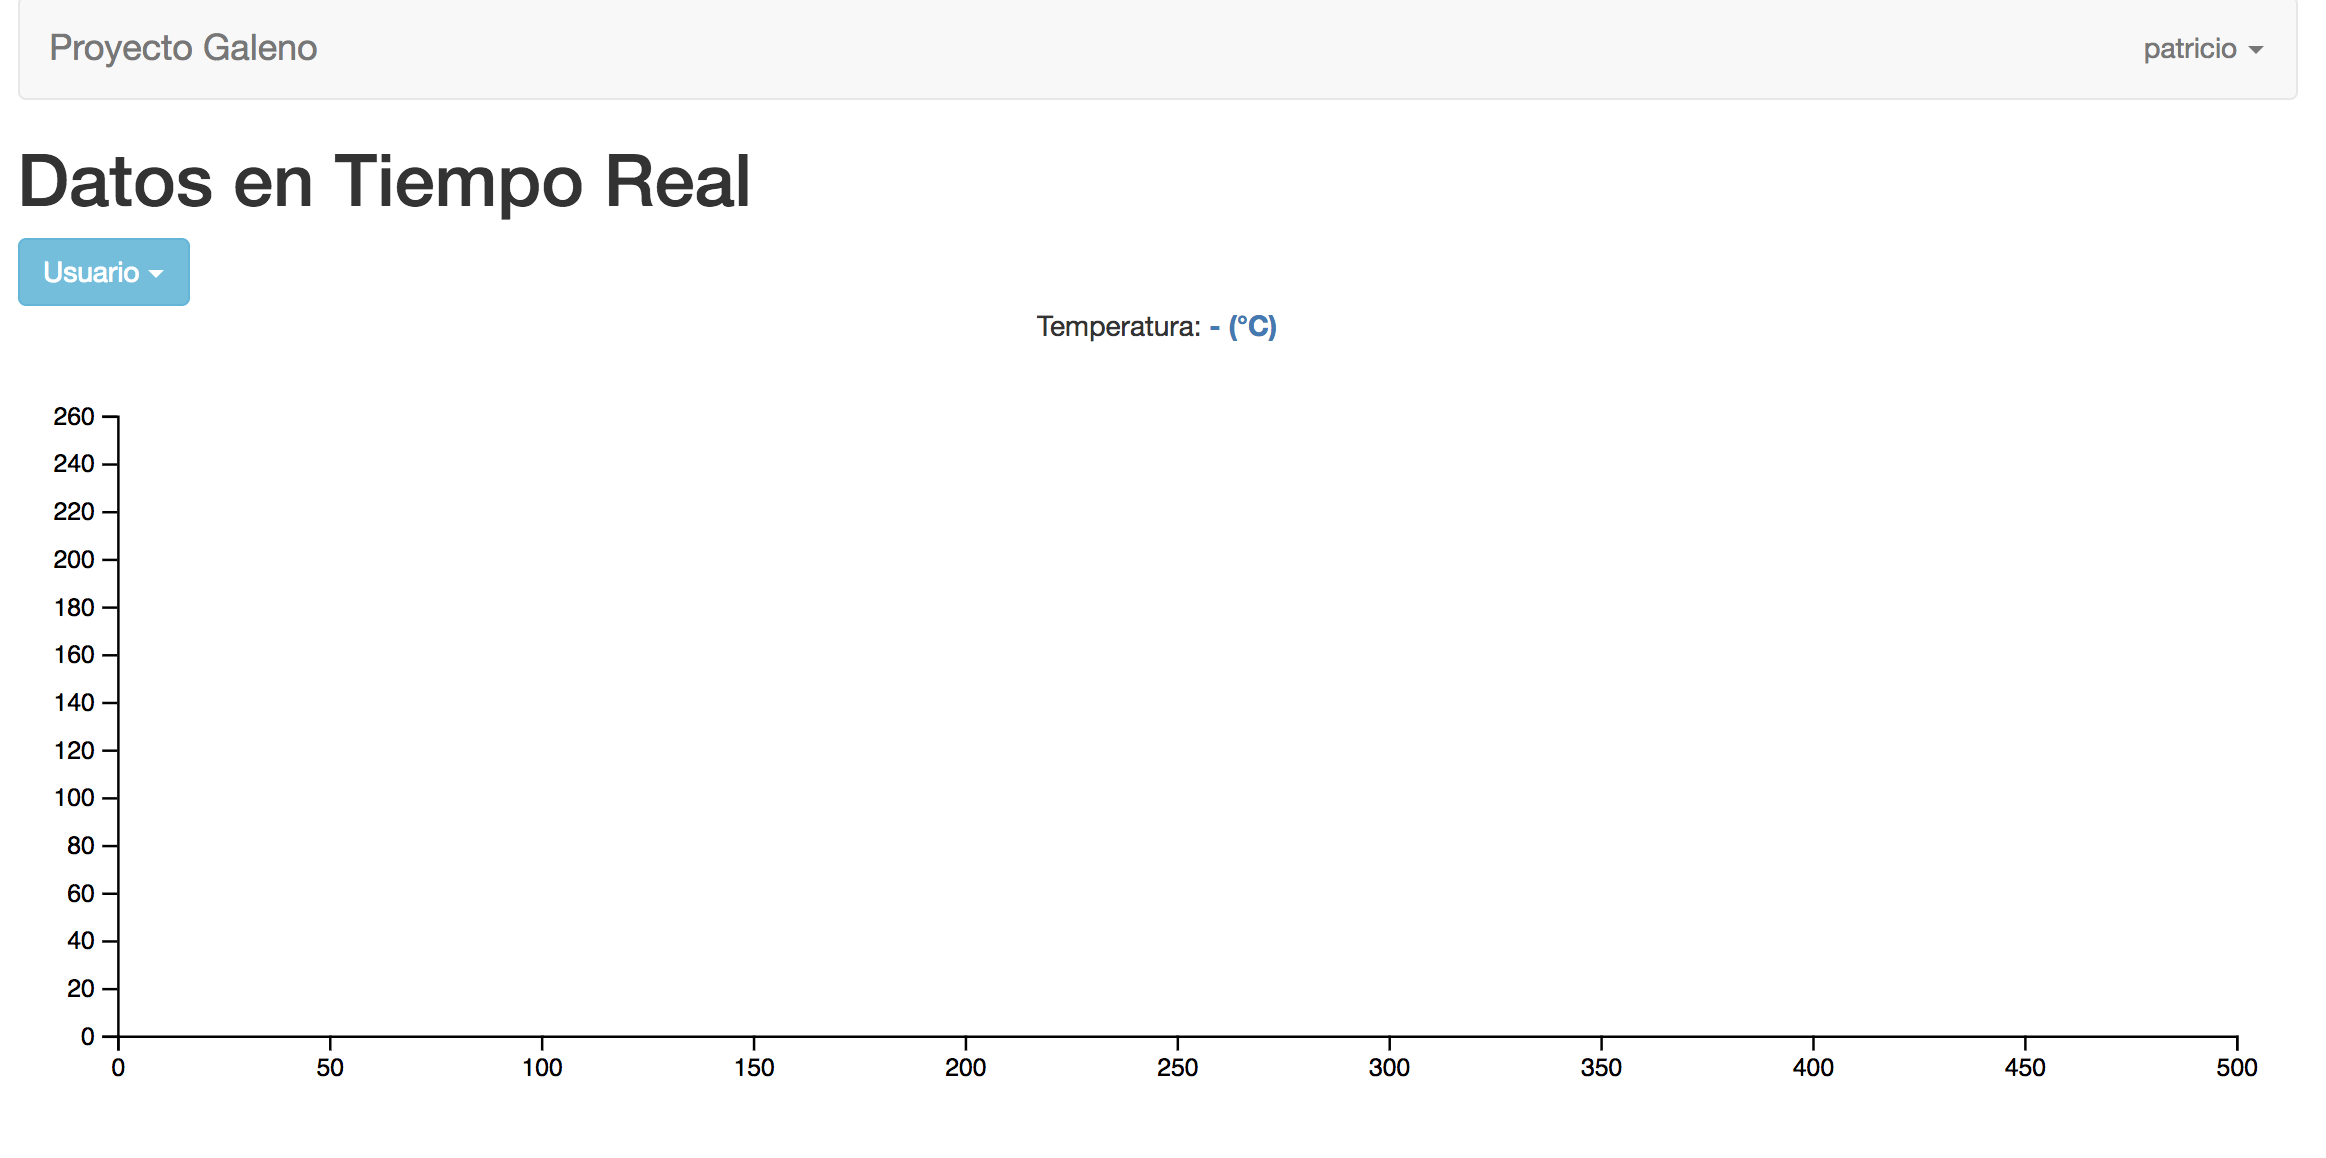
\includegraphics[scale=0.3]{figuras/protof/normal.png}
	\caption{Pantalla principal de un usuario normal}
	\label{normal}
\end{figure}

\begin{figure}[H]
	\centering
	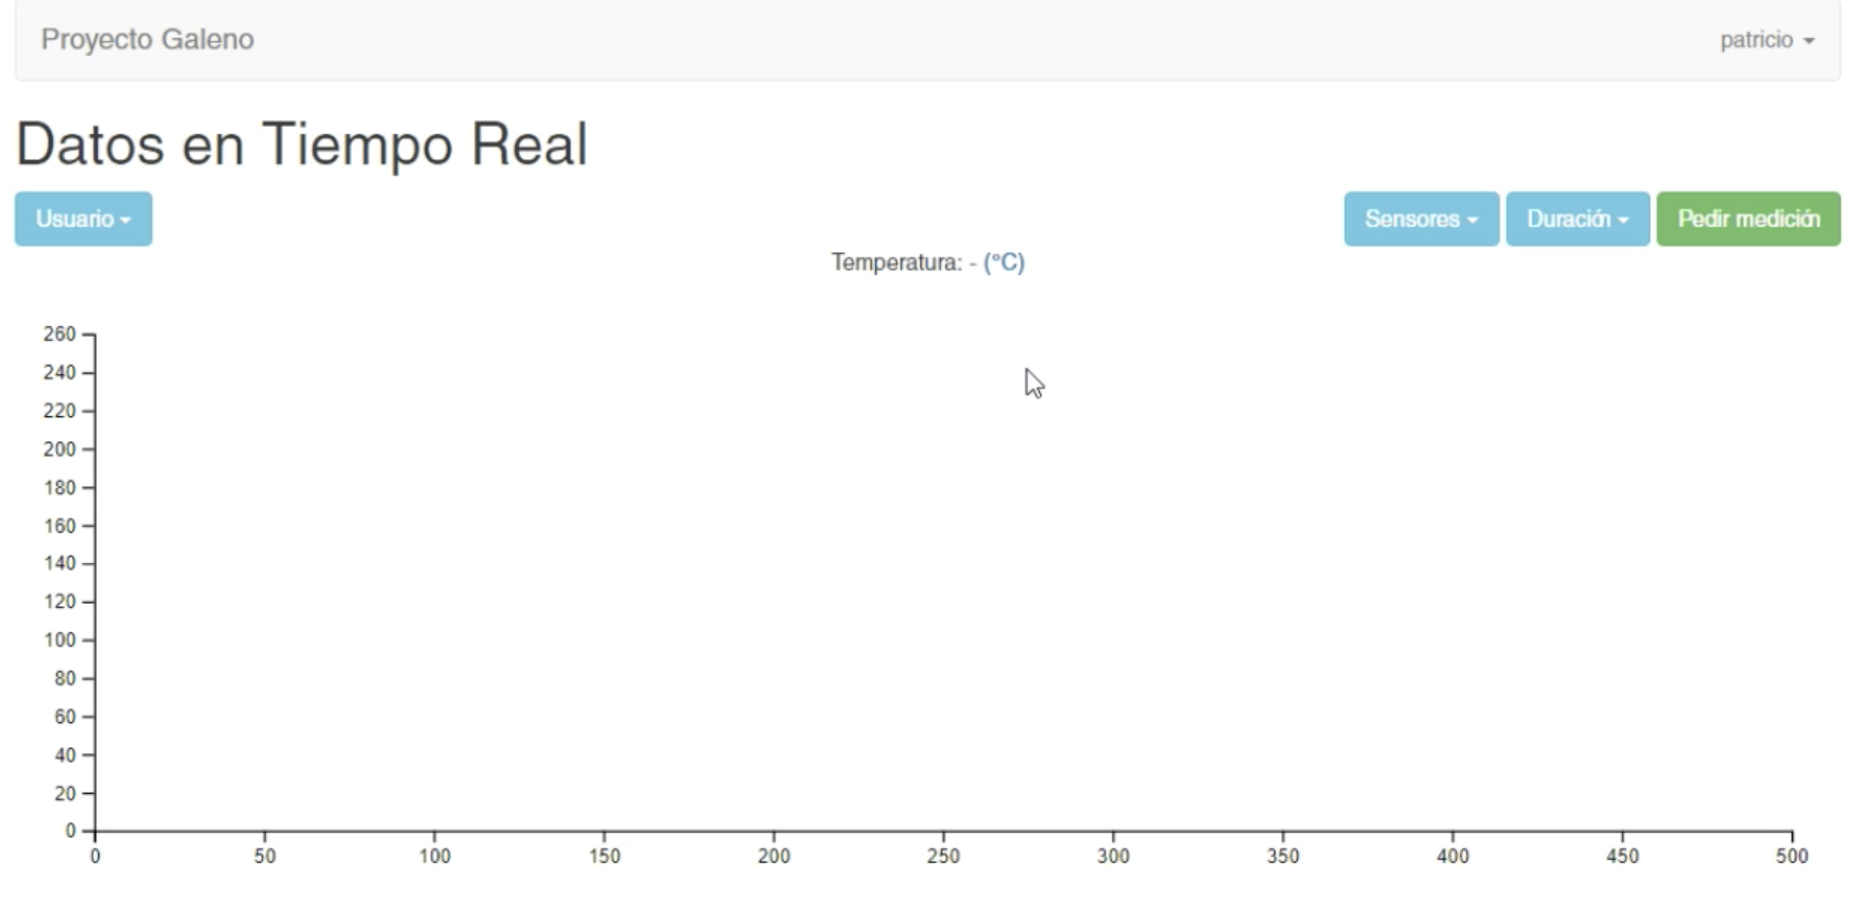
\includegraphics[scale=0.4]{figuras/protof/total.png}
	\caption{Pantalla principal de un usuario con acceso total}
	\label{total}
\end{figure}

Como se puede observar en las figuras anteriores, la única diferencia entre las distintas cuentas son los botones que especifican una medición (sensores y duración).

De la pantalla principal se pueden destacar el control de ingreso en la parte superior derecha, el botón de la izquierda concerniente a la selección del usuario a visualizar, a la derecha los botones de la medición y el gráfico principal con el ECG junto a la temperatura sobre este último.

\begin{figure}[H]
	\centering
	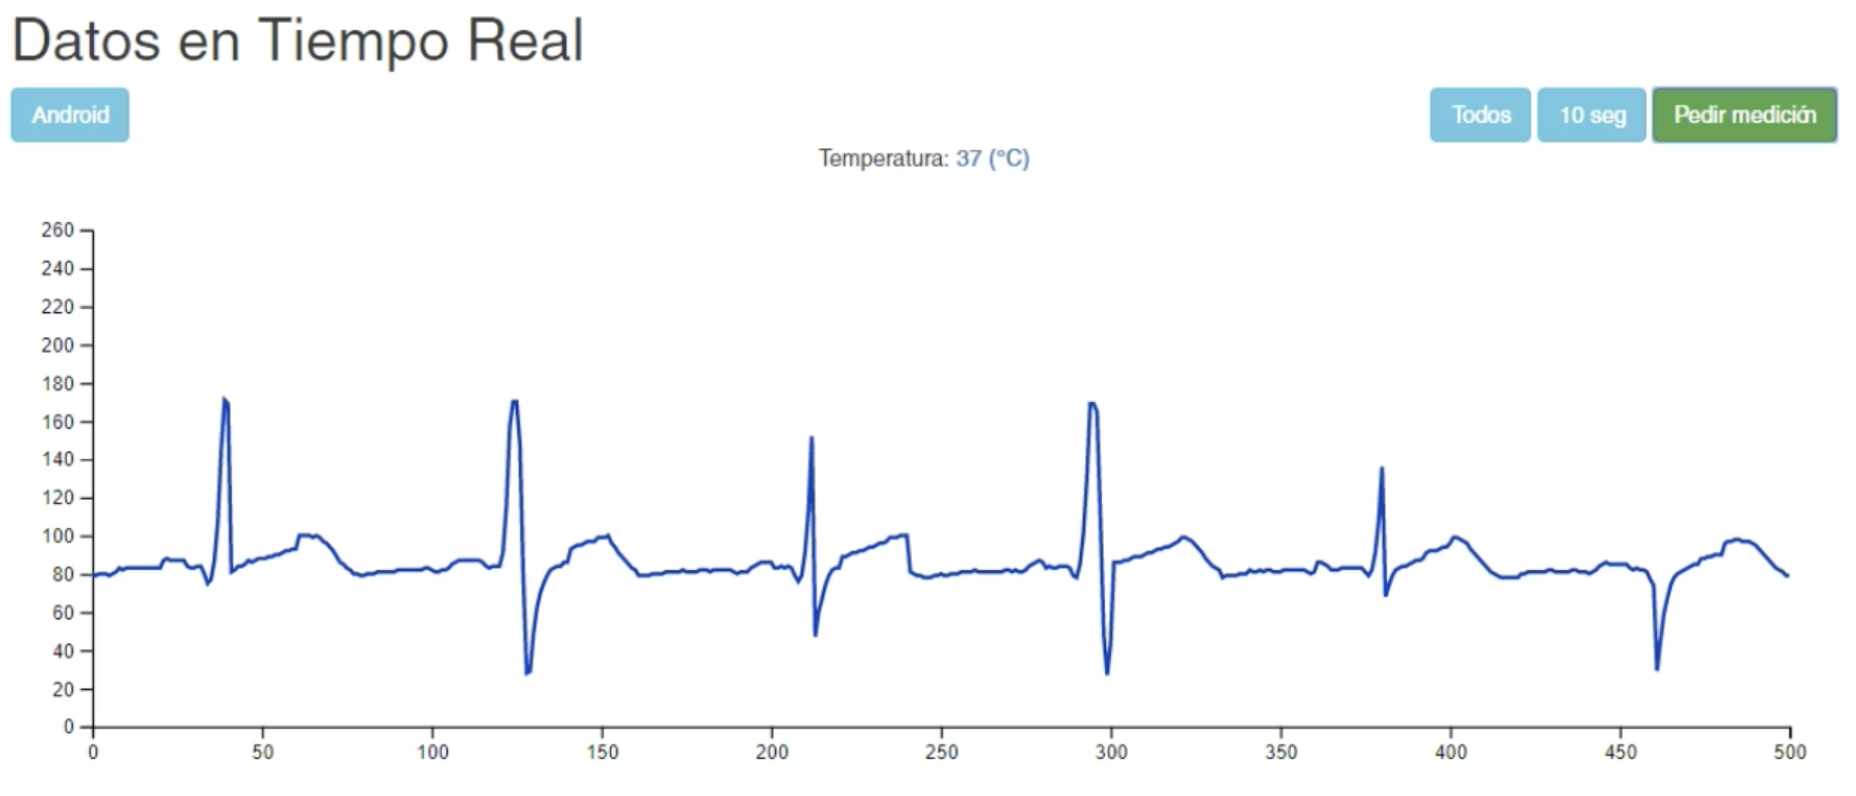
\includegraphics[scale=0.4]{figuras/protof/medicion.png}
	\caption{Medición de ambos sensores en tiempo real}
	\label{medicion}
\end{figure}

Como se puede observar en la figura \ref{medicion}, el gráfico resultante se encuentra desfasado en unos 2 segundos respecto al que se muestra en la pantalla de la aplicación. Todo dato que es mostrado, es almacenado tanto de forma local (Android - Realm) como en el servidor web (Meteor - MongoDB).

\begin{figure}[H]
	\centering
	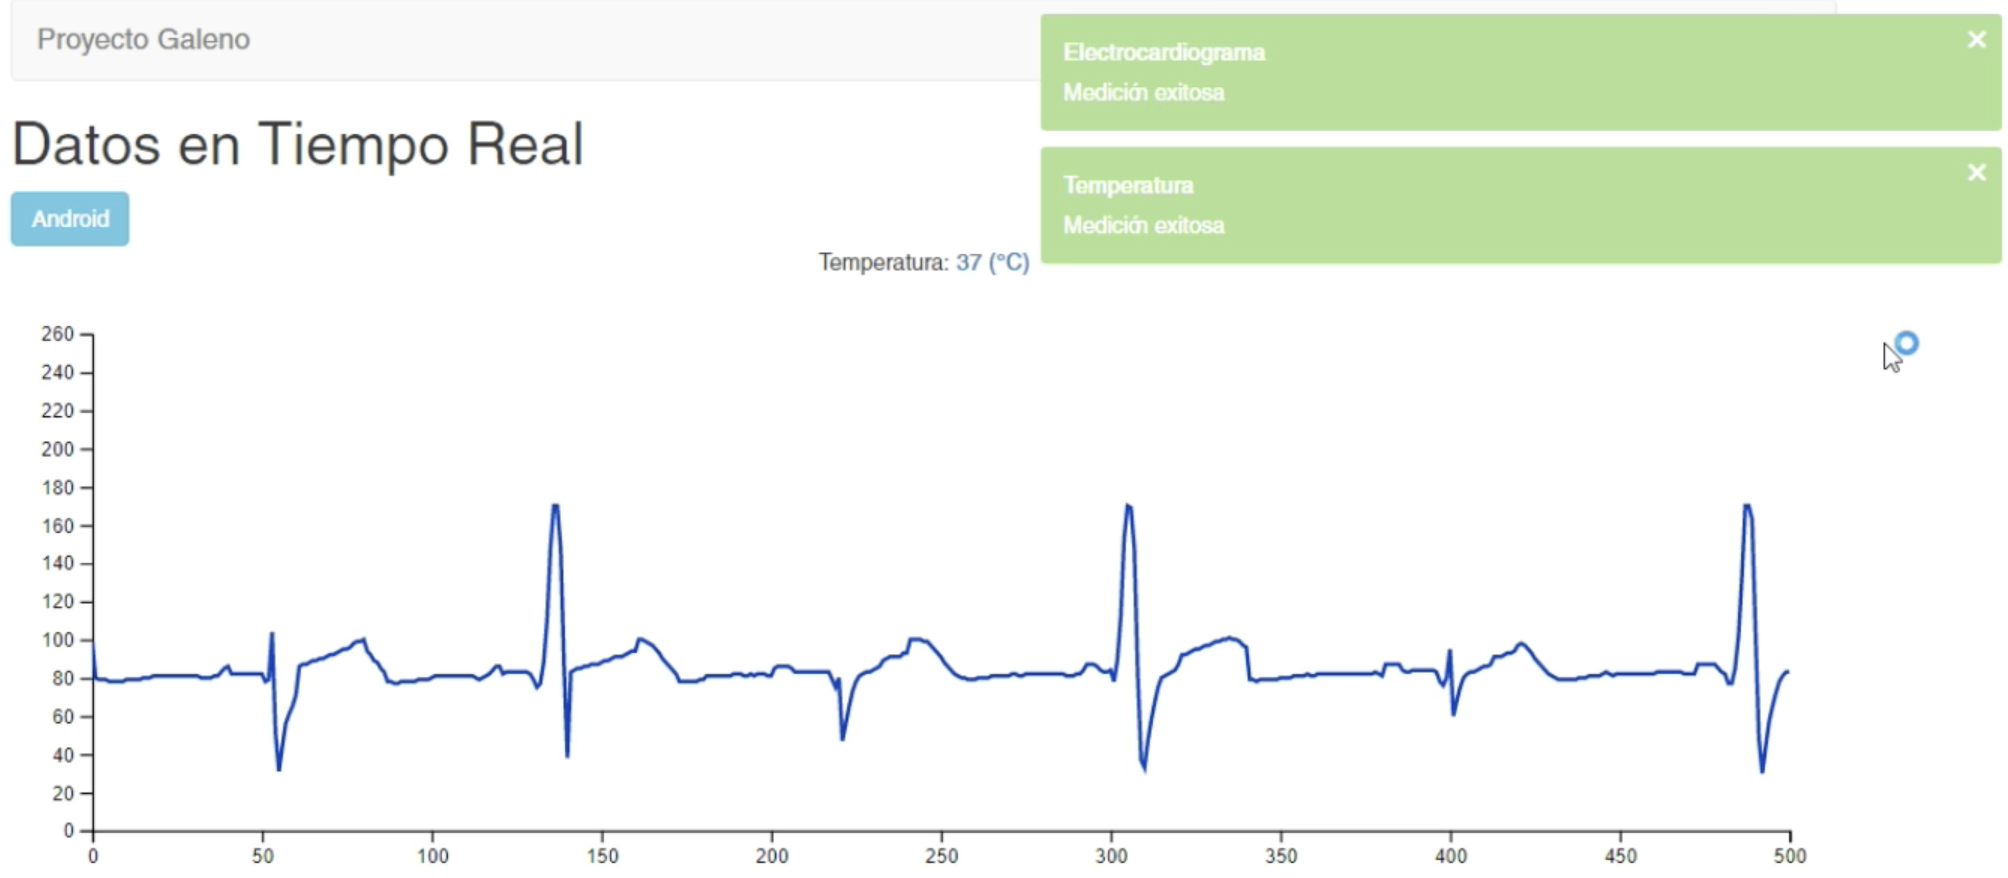
\includegraphics[scale=0.4]{figuras/protof/medicionPc.png}
	\caption{Medición de ambos sensores en tiempo real por página Web}
	\label{medicionPc}
\end{figure}


\begin{figure}[H]
	\centering
	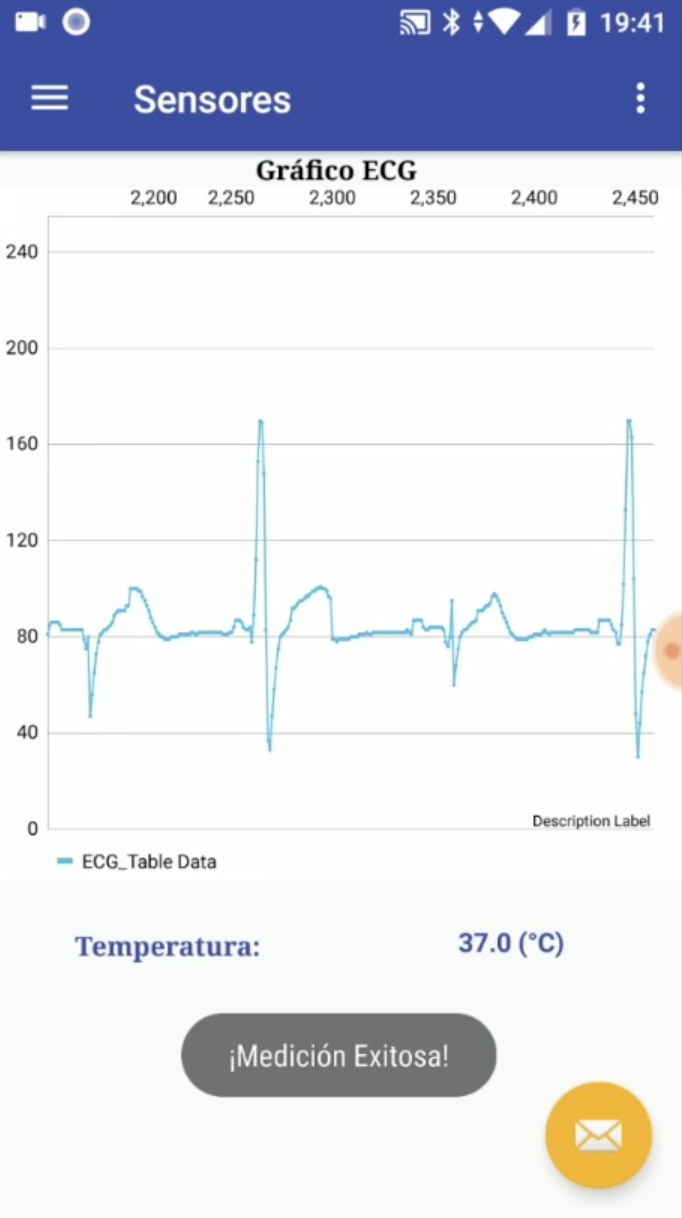
\includegraphics[scale=0.4]{figuras/protof/medicionApp.png}
	\caption{Medición de ambos sensores en tiempo real por aplicación Android}
	\label{medicionApp}
\end{figure}

En las figurlas \ref{medicionPc} y \ref{medicionApp} se puede observar una misma medición siendo finalizada exitosamente, en la que por un lado en la página web se presentan las dos notificaciones asociadas a cada sensor y en la aplicación un Toast (común mensaje flotante en Android) indicando su término correcto.

Es importante destacar que de fallar la medición, ya sea por uno o por los dos sensores (conteo total de datos enviados distintos entre microcontrolador y aplicación) ésta se reiniciará automáticamente, sin intervención del usuario y los datos almacenados en las distintas bases de datos serán borrados (como cabe esperar en un caso de error).

Por último, si se es riguroso se puede observar una temperatura bastante exacta en las distintas figuras presentadas, esto es debido a que el sensor de temperatura presentó problemas en su última utilización. A raíz de esto, se reemplazó su valor desde el microcontrolador con un valor fijo, esto último para validar el flujo completo de dicho sensor, aislando así el problema solo al sensor y no a todo el flujo de comunicación.


